\documentclass[10pt]{article}
\usepackage{tikz}
\usetikzlibrary{shapes.misc}
\usepackage[margin=0cm]{geometry}
\pagestyle{empty}
\tikzstyle{every node}=[cross out, draw, red]

\begin{document}

\vspace*{\fill}
\begin{center}
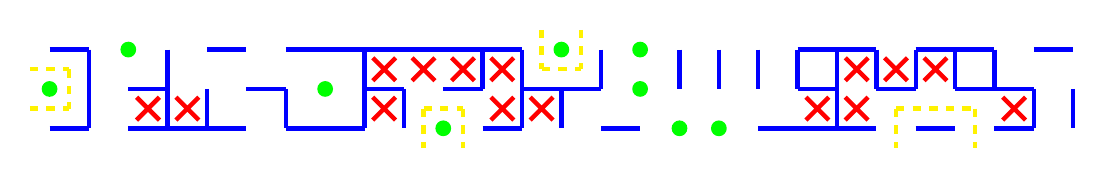
\begin{tikzpicture}[x=0.5cm, y=-0.5cm, ultra thick, blue]
% Walls
    \draw (0,0) -- (1,0);
    \draw (4,0) -- (5,0);
    \draw (6,0) -- (12,0);
    \draw (19,0) -- (21,0);
    \draw (22,0) -- (24,0);
    \draw (25,0) -- (26,0);
    \draw (2,1) -- (3,1);
    \draw (5,1) -- (6,1);
    \draw (8,1) -- (9,1);
    \draw (10,1) -- (11,1);
    \draw (12,1) -- (14,1);
    \draw (19,1) -- (20,1);
    \draw (21,1) -- (22,1);
    \draw (23,1) -- (25,1);
    \draw (0,2) -- (1,2);
    \draw (2,2) -- (5,2);
    \draw (6,2) -- (8,2);
    \draw (11,2) -- (12,2);
    \draw (14,2) -- (15,2);
    \draw (18,2) -- (21,2);
    \draw (22,2) -- (23,2);
    \draw (24,2) -- (25,2);
    \draw (1,0) -- (1,2);
    \draw (3,0) -- (3,2);
    \draw (4,1) -- (4,2);
    \draw (6,1) -- (6,2);
    \draw (8,0) -- (8,2);
    \draw (9,1) -- (9,2);
    \draw (11,0) -- (11,1);
    \draw (12,0) -- (12,2);
    \draw (13,1) -- (13,2);
    \draw (14,0) -- (14,1);
    \draw (16,0) -- (16,1);
    \draw (17,0) -- (17,1);
    \draw (18,0) -- (18,1);
    \draw (19,0) -- (19,1);
    \draw (20,0) -- (20,2);
    \draw (21,0) -- (21,1);
    \draw (22,0) -- (22,1);
    \draw (23,0) -- (23,1);
    \draw (24,0) -- (24,1);
    \draw (25,1) -- (25,2);
    \draw (26,1) -- (26,2);
% Pillars
    \fill[green] (2,0) circle(0.2);
    \fill[green] (13,0) circle(0.2);
    \fill[green] (15,0) circle(0.2);
    \fill[green] (0,1) circle(0.2);
    \fill[green] (7,1) circle(0.2);
    \fill[green] (15,1) circle(0.2);
    \fill[green] (10,2) circle(0.2);
    \fill[green] (16,2) circle(0.2);
    \fill[green] (17,2) circle(0.2);
% Inner points in accessible cul-de-sacs
    \node at (8.5,0.5) {};
    \node at (9.5,0.5) {};
    \node at (10.5,0.5) {};
    \node at (11.5,0.5) {};
    \node at (20.5,0.5) {};
    \node at (21.5,0.5) {};
    \node at (22.5,0.5) {};
    \node at (2.5,1.5) {};
    \node at (3.5,1.5) {};
    \node at (8.5,1.5) {};
    \node at (11.5,1.5) {};
    \node at (12.5,1.5) {};
    \node at (19.5,1.5) {};
    \node at (20.5,1.5) {};
    \node at (24.5,1.5) {};
% Entry-exit paths without intersections
    \draw[dashed, yellow] (-0.5,0.5) -- (0.5,0.5);
    \draw[dashed, yellow] (12.5,0.5) -- (13.5,0.5);
    \draw[dashed, yellow] (-0.5,1.5) -- (0.5,1.5);
    \draw[dashed, yellow] (9.5,1.5) -- (10.5,1.5);
    \draw[dashed, yellow] (21.5,1.5) -- (23.5,1.5);
    \draw[dashed, yellow] (0.5,0.5) -- (0.5,1.5);
    \draw[dashed, yellow] (9.5,1.5) -- (9.5,2.5);
    \draw[dashed, yellow] (10.5,1.5) -- (10.5,2.5);
    \draw[dashed, yellow] (12.5,-0.5) -- (12.5,0.5);
    \draw[dashed, yellow] (13.5,-0.5) -- (13.5,0.5);
    \draw[dashed, yellow] (21.5,1.5) -- (21.5,2.5);
    \draw[dashed, yellow] (23.5,1.5) -- (23.5,2.5);
\end{tikzpicture}
\end{center}
\vspace*{\fill}

\end{document}
